\section{Additional Experiments}
\label{sec:additional-experiments}

In this section we present additional and extended results from the main section.

\subsection{Power and False Discoveries for Multiple Features}%
\label{sec:power-fdr-multiple}

Here, we study how the power of correctly detecting \(k=10\) signals under \(q_j\) linearly
spaced in \([0.5, 0.99]\)~(\Cref{fig:binary-power}). We set \(\beta^*_j = 2\) for each of
the signals, use \(n = 100\,000\), and let \(\sigma_\varepsilon = 1\). The level of
regularization is set to \(\lambda_1 = n 4^\delta/10\). As we can see, the power is
directly related to \(q_j\) and for unbalanced features stronger the higher the choice of
\(\delta\) is.

We also consider a version of the same setup, but with \(p\) linearly spaced in \([20,
    100]\) and compute normalized mean-squared error (NMSE) and false discovery rate
(FDR)~(\Cref{fig:binary-fdr-mse}). As before, we let \(k = 10\) and consider three
different levels of class imbalance. The remaining \(p-k\) features have class balances
spaced evenly on a logarithmic scale from 0.5 to 0.99. Unsurprisingly, the increase in
power gained from selecting \(\delta = 1\) imposes increased false discovery rates. We also
see that the mean-squared error depends on class balance. In line with our previous
results, \(\delta \in \{0, 1/2\}\) appears to work well for balanced features whilst
\(\delta = 1\) works better when there are large imbalances. In the case when \(q_j =
0.99\), the model under scaling with \(\delta = 0\) does not detect any of the true
signals.

\begin{figure}[htpb]
  \centering
  \subfigure[%
    The power (probability of detecting all true signals) of the lasso. In our
    orthogonal setting, power is constant over \(p\), which is why we have
    omitted the parameter in the plot. \label{fig:binary-power}
  ]{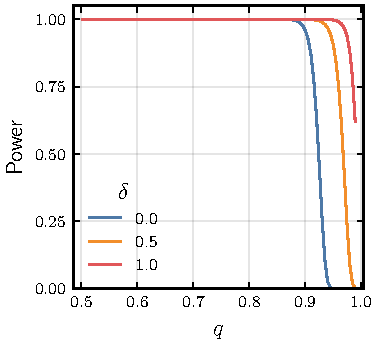
\includegraphics[]{power.pdf}}\hfill%
  \subfigure[%
    NMSE and FDR: the rate of coefficients incorrectly set to non-zero (false
    discoveries) to the total number of estimated coefficients that are nonzero
    (discoveries).
    \label{fig:binary-fdr-mse}]{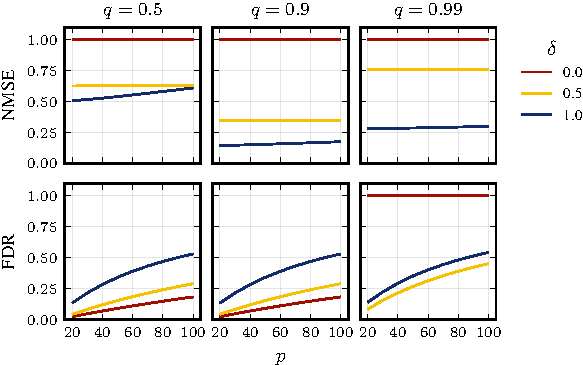
\includegraphics[]{fdr_mse.pdf}}%%
  \caption{%
    Normalized mean-squared error (NMSE), false discovery rate (FDR), and power
    for a lasso problem with \(k = 10\) true signals (nonzero \(\beta_j^*\)),
    varying \(p\), and \(q_j \in [0.5, 0.99]\). The noise level is set at
    \(\sigma_\varepsilon = 1\) and \(\lambda_1 = 0.02\).
  }
\end{figure}

\subsection{Support Size and Predictive Performance}
\label{sec:predictive-performance-support}

In this section we analyze the support size of the lasso estimates for the experiment in
\Cref{sec:experiments-predictive-performance}. In \Cref{fig:hyperopt-support}, we have, in
addition to NMSE on the validation set, also plotted the size of the support of the lasso
(cardinality of the set of features that have corresponding nonzero coefficients). Here we
only show results for \(\delta \in \{0, 1/2, 1\}\).

\begin{figure}[htpb]
  \centering
  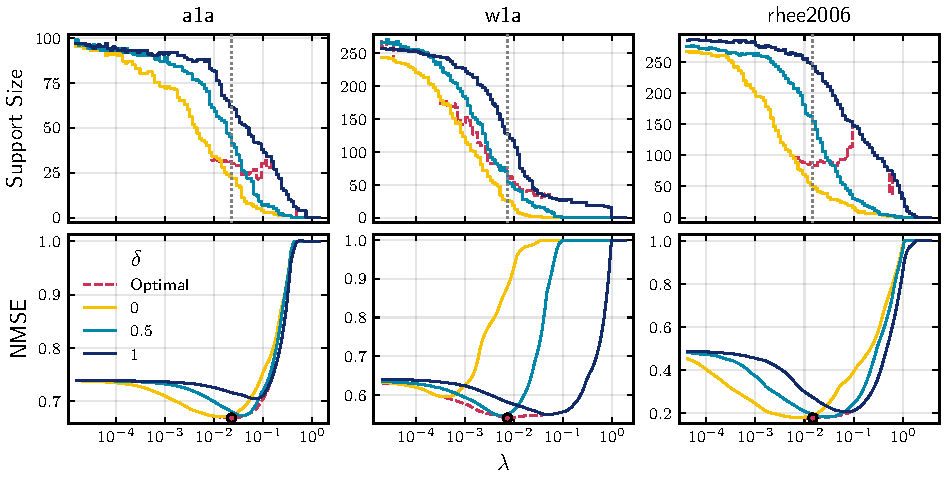
\includegraphics[]{hyperopt_paths.pdf}
  \caption{%
    Support size and normalized mean-squared error (NMSE) for the validation set for the lasso
    fit to datasets \data{rhee2006}, \data{eunite2001}, and \data{triazines} across combinations of
    \(\delta\) and \(\lambda\). The optimal \(\delta\) is marked with dashed black lines and
    the best combination of \(\delta\) (among 0, 1/2, and 1) and \(\lambda\) is shown as a dot.
  }
  \label{fig:hyperopt-support}
\end{figure}

\subsection{Predictive Performance for Simulated Data}%
\label{sec:predictive-performance-simulated}

In this experiment, we consider predictive performance in terms of mean-squared error of
the lasso and ridge regression given different levels of class balance (\(q_j \in \{0.5,
0.9, 0.99\}\)), signal-to-noise ratio, and normalization (\(\delta\)). All of the features
are binary, but here we have used \(n=300\) and \(p = \num{1000}\). The \(k=10\) first
features correspond to true signals with \(\beta^*_j = 1\) and all have class balance
\(q\). To set signal-to-noise ratio levels, we rely on the same choice as in
\citet{hastie2020} and use a log-spaced sequence of values from 0.05 to 6. We use standard
hold-out validation with equal splits for training, validation, and test sets. And we fit a
full lasso path, parameterized by a log-spaced grid of 100 values\footnote{This is a
  standard choice of grid, used for instance by \citet{friedman2010}}, from
\(\lambda_\text{max}\) (the value of \(\lambda\) at which the first feature enters the
model) to \(10^{-2}\lambda_\text{max}\) on the training set and pick \(\lambda\) based on
validation set error. Then we compute the hold-out test set error and aggregate the results
across 100 iterations.

The results~(\Cref{fig:binary-sim}) show that the optimal normalization type in terms of
prediction power depends on the class balance of the true signals. If the imbalance is
severe, then we gain by using \(\delta=1/2\) or \(1\), which gives a chance of recovering
the true signals. If everything is balanced, however, then we do better by not scaling. In
general, \(\delta=1/2\) works well for these specific combinations of settings.

\begin{figure}[htpb]
  \centering
  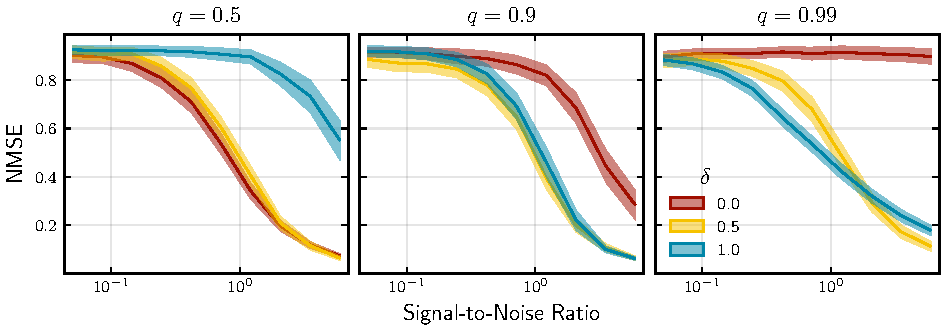
\includegraphics[]{binary_data_sim.pdf}
  \caption{%
    Normalized mean-squared prediction error in a lasso model for different types of
    normalization (\(\delta\)), types of class imbalances (\(q_j\)), and signal-to-noise ratios
    (0.05 to 6) in a dataset with \(n=300\) observations and \(p = \num{1000}\) features. The
    error is aggregated test-set error from hold-out validation with \(100\) observations in
    each of the training, validation, and test sets. The plot shows means and Student's
    \(t\)-based 95\% confidence intervals. } \label{fig:binary-sim}
\end{figure}

\subsection{Comparisons of Normalization Methods on Real Data}
\label{sec:normalization-tuning}

In this section we present an extended and modified version of the experiment in
\Cref{sec:experiments-predictive-performance}, by considering several additional datasets,
including datasets with binary responses to which we have fit \(\ell_1\) and
\(\ell_2\)-regularized logistic regression. Instead of only considering parameterization
over \(\delta\), we also extend the benchmarks to cover additional normalization types. For
each of the datasets, we have fit the lasso and ridge for 10-times repeated 10-folds
cross-validation over a grid of \(\lambda\) and normalization method. In the case of the
method we call ``ours'', we have extended the grid over \(\delta\) as well, and return the
results for the \(\delta\) with lowest error.

The results are shown in \Cref{fig:method-comparison} and show that the optimal choice of
normalization depends on the dataset and type of model. Using our strategy, which
corresponds to standardization for continuous data and hyper-tuning over \(\delta\) attains
best results for most of the datasets, only ever slightly worse than the best performing
method. Among the methods, \(\ell_1\) normalization seems to perform poorly in general.
Given the fact that that it corresponds to variance-scaling for binary data, which we have
shown results in considerable variance, this is not particularly surprising.

\begin{figure*}[htpb]
  \centering
  \subfigure[%
    Results for the lasso
    % \label{fig:method-comparison-lasso}
  ]{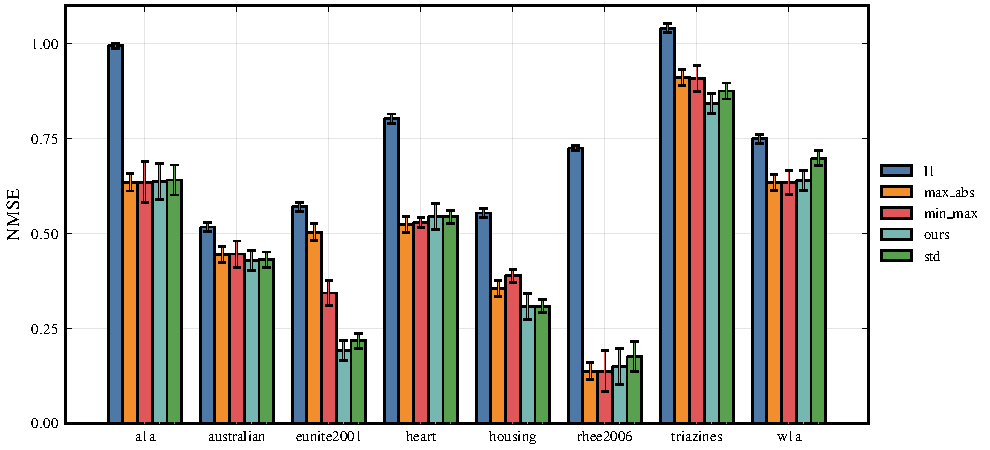
\includegraphics[]{method_comparison_lasso.pdf} }
  \subfigure[%
    Results for ridge regression
    % \label{fig:method-comparison-ridge}
  ]{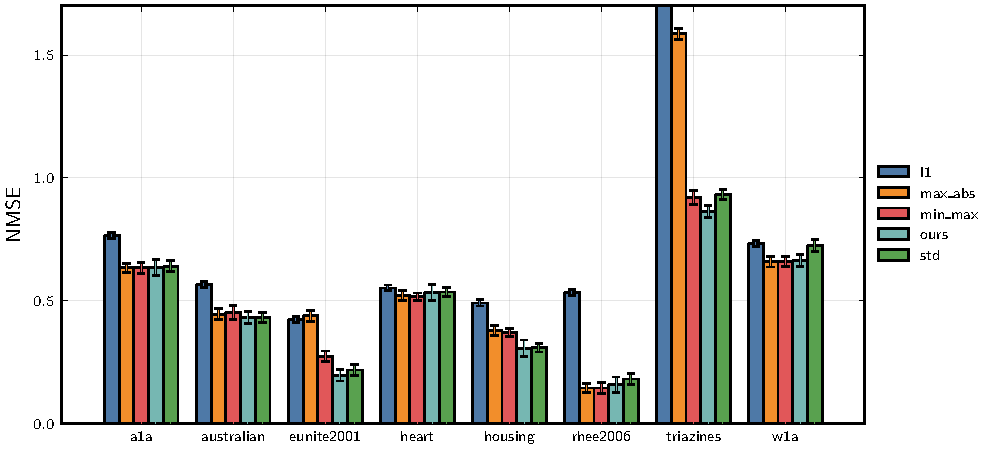
\includegraphics[]{method_comparison_ridge.pdf}}
  \caption{%
    Cross-validation error from 10-times repeated 10-folds cross validation for the lasso and ridge
    and various datasets and normalization strategies. The error is normalized mean-squared
    error (NMSE). In the case of datasets \data{a1a}, \data{w1a}, \data{heart}, \data{w1a},
    and \data{australian}, we have fit regularized logistic regression and
    otherwise regularized linear regression. The error bars show 95\% confidence intervals.
  }
  \label{fig:method-comparison}
\end{figure*}

\subsection{Dichotomization and Feature Selection}
\label{sec:dichotomization}

In this experiment, we attempt to study the effect of normalization choice in feature
selection on datasets with dichotomized features and the following dichotomization scheme
to convert the continuous features to binary.

Each variable was converted to a binary feature by comparing against threshold based on
either historical standards, regulatory guidelines, or domain-specific knowledge of urban
housing factors in the 1970s~(\Cref{tab:dichotomization}).

\begin{table}[htbp]
  \centering
  \caption{
    Dichotomization procedure and linear regression coefficients for the
    features of the Boston housing dataset used in the experiment in
    \Cref{sec:dichotomization}.
  }
  \label{tab:dichotomization}
  \begin{tabular}{
      l
      p{9.5cm}
      S[table-format=-1.2,round-mode=places,round-precision=2]
      S[table-format=0.2,round-mode=places,round-precision=2]
    }
    \toprule
    Feature             & Dichotomization Rule                                                                         & $\hat{\bm{\beta}}_j^\text{OLS}$ & $q_j$     \\
    \midrule
    Crime Rate          & Above/below national U.S. average crime rate (1970--1971)                                    & -1.872296271668692              & 0.8992094 \\
    Zoning              & Presence/absence of large lot zoning (residential lots over 25,000 sq.ft)                    & 1.956883402813590               & 0.2648221 \\
    Business            & Residential vs industrial areas (below/above 10\% non-retail business acres)                 & -2.41422163254033               & 0.4664031 \\
    Charles River       & Original binary feature (borders river or not)                                               & 5.118087353331369               & 0.0691699 \\
    NOx Concentration   & Above/below EPA air quality standard for NOx (53 parts per billion)                          & -2.607920261778666              & 0.5177865 \\
    Rooms               & Above/below typical family dwelling size (more/less than 6 rooms)                            & 3.486474827676998               & 0.6581027 \\
    Age                 & Newer vs historic housing (less/more than 50\% built before 1940)                            & -1.101306211297333              & 0.7094861 \\
    Distance            & Close vs far from employment centers (less/more than 5 miles)                                & -4.762540742210745              & 0.2667984 \\
    Highway Access      & Limited vs good highway access (accessibility index below/above 20)                          & 1.250197827256583               & 0.2608695 \\
    Property Tax        & Below/above Massachusetts average property tax rate (approximately \$12 per \$1000 in 1970s) & -7.347485535327863              & 0.9664031 \\
    Pupil-Teacher Ratio & Below/above recommended educational value (16 students per teacher)                          & -6.567220592441502              & 0.8320158 \\
    Demographics        & More/less diverse population (above/below 85\% white)                                        & 3.245798334030099               & 0.9486166 \\
    Lower Status        & Middle-class vs lower-income areas (below/above 15\% lower status population)                & -7.240796759180348              & 0.3201581 \\
    \bottomrule
  \end{tabular}
\end{table}

Having dichotomized the data, we then first fit a standard linear regression model to the
data, and use this as a proxy for feature importance. Then, for three types of
normalization: \(\ell_1\)-normalization (\(\delta=1\)), standardization, and min--max
normalization, we fit a lasso model to the data and compute ranks of the features by
checking at which point they enter the model.

Finally, we compare the ranks of the features in the lasso model to the ranks of the
coefficients from the standard linear regression model, using the latter as the reference.
We use four different metrics to compare the ranks: Spearman's rank correlation, Kendall's
\(\tau\), mean absolute difference, and normalized discounted cumulative gain (NDCG). The
results are presented in \Cref{tab:method_comparison}. The results show that the
normalization method using \(\ell_1\)-normalization (\(\delta = 1\)) best corresponds to
the ranks of the linear regression coefficients.

\begin{table}[htbp]
  \centering
  \caption{
    Comparison between ranks of ordinary least-squares coefficients and ranks
    given by the order of model entry along the lasso path for the Boston
    housing dataset. The metrics used are Spearman's and Kendall's rank
    correlations, normalized discounted cumulative gain (NDCG), and mean
    absolute difference (MAD). Best values are marked in blod face. For all
    measures except MAD, higher values are better.
  }%
  \label{tab:method_comparison}
  \begin{tabular}{l S[table-format=1.4,detect-weight] S[table-format=1.4] S[table-format=1.4]}
    \toprule
    Metric   & {\(\ell_1\)-Normalization} & {Standardization} & {Min--Max/Max--Abs} \\
    \midrule
    Spearman & \best 0.7308               & 0.5714            & 0.5                 \\
    Kendall  & \best 0.5128               & 0.4359            & 0.3846              \\
    MAD      & \best 2.0                  & 2.7692            & 3.0769              \\
    NDCG     & \best 0.9515               & 0.9351            & 0.9186              \\
    \bottomrule
  \end{tabular}
\end{table}
